\documentclass[11pt]{article}
\usepackage{amsthm}
\usepackage{amsmath}
\usepackage{amssymb}
\usepackage{amsfonts}
\usepackage{graphicx}
\usepackage{color}
\usepackage{enumerate}
\usepackage{amscd}

\usepackage{longtable}


\usepackage{algorithm}
\usepackage{algorithmicx}
\usepackage{algpseudocode}

\usepackage[sort&compress,numbers]{natbib}


\usepackage{mathptmx}
%\usepackage[scaled]{helvet}
%\renewcommand\familydefault{\sfdefault}
%\usepackage[T1]{fontenc}





\usepackage{tikz-cd}
\usepackage[hyphens]{url}
\urlstyle{same}

\usepackage{wrapfig}
\usepackage{mathrsfs}
\usepackage{mdframed}

\usepackage{dsfont} % blackboard numerals

\usepackage{geometry}
\geometry{margin=0.75in}

\usepackage{setspace}

%\usepackage{endfloat}



\newcommand{\R}{\mathbb{R}}
\newcommand{\E}{\mathbb{E}}
\newcommand{\Econd}{\E_{\Yij|\Yinj,\xinj}}
\newcommand{\EXY}{\E_{\Yinj,\xinj}}
\newcommand{\Prob}{\mathbb{P}}
\newcommand{\LDGP}{L^{\text{DGP}}}
\newcommand{\lDGP}{l^{\text{DGP}}}
\newcommand{\lcox}{l^{\text{Cox}}}
\newcommand{\lpois}{l^{\text{Pois}}}
\newcommand{\hazt}{\lambda_{ij}(t)}
\newcommand{\Yij}{Y_{ij}}
\newcommand{\Yik}{Y_{ik}}
\newcommand{\Yinj}{Y_{i-j}(t)}


\newcommand{\cDE}{\text{\it cDE}}
\newcommand{\mDE}{\text{\it mDE}}
\newcommand{\mPE}{\text{\it mPE}}

\newcommand{\xij}{x_{ij}}
\newcommand{\xik}{x_{ik}}
\newcommand{\xinj}{x_{i-j}}
\newcommand{\tij}{t_{ij}}
\newcommand{\tik}{t_{ik}}
\newcommand{\T}{\mathbf{T}}
\newcommand{\V}{\mathbf{V}}
\newcommand{\W}{\mathbf{W}}
\newcommand{\X}{\mathbf{X}}
\newcommand{\Y}{\mathbf{Y}}
\newcommand{\Z}{\mathbf{Z}}
\newcommand{\bH}{\mathbf{H}}
\newcommand{\h}{\mathbf{h}}
\newcommand{\x}{\mathbf{x}}
\newcommand{\y}{\mathbf{y}}
\newcommand{\z}{\mathbf{z}}
\newcommand{\w}{\mathbf{w}}

\newcommand{\bomega}{\boldsymbol{\omega}}
\newcommand{\bxi}{\boldsymbol{\xi}}
\newcommand{\btheta}{\boldsymbol{\theta}}
\newcommand{\bphi}{\boldsymbol{\phi}}
\newcommand{\balpha}{\boldsymbol{\alpha}}
\newcommand{\betapois}{\hat{\beta}_{\text{Pois}}}
\newcommand{\betacox}{\hat{\beta}_{\text{Cox}}}
\newcommand{\betaDGP}{\hat{\beta}_{\text{DGP}}}
\newcommand{\betaPA}{\hat{\beta}_{\text{PA}}}
\newcommand{\er}{\text{error}}
\newcommand{\omegastar}{\omega^{\textstyle{*}}}
\newcommand{\etastar}{\eta^{\textstyle{*}}}

\newcommand{\dx}[1]{\ \text{d} #1}
\newcommand{\indicator}[1]{\mathds{1}\!\left\{ #1 \right\}}
\newcommand{\indep}{\ \rotatebox[origin=c]{90}{$\models$}\ }
\newcommand{\nindep}{\not\!\perp\!\!\!\perp}

\newcommand{\comment}[1]{[\textcolor{red}{#1}]}

\newtheorem{thm}{Theorem}[section]
\newtheorem{prop}{Proposition}
\newtheorem{cor}{Corollary}
\newtheorem{lem}{Lemma}
\newtheorem{defn}{Definition}

\setlength{\bibsep}{0.0pt}
\setlength{\parskip}{1em}
\setlength{\parindent}{0.0pt}


\allowdisplaybreaks


% Blinding for peer review: set to 1
\newcommand{\blind}{0}



\title{COVID-19 projections for reopening Connecticut}

\author{
  Forrest W. Crawford$^{1,2,3,4}$,
  Olga Morozova$^{1}$, 
  and
  Zehang Richard Li$^1$
  \\[1em]
\small 1. Department of Biostatistics, Yale School of Public Health \\
\small 2. Department of Statistics \& Data Science, Yale University \\
\small 3. Department of Ecology \& Evolutionary Biology, Yale University \\
\small 4. Yale School of Management }



%%%%%%%%%%%%%%%%%%%%%%%%%%%%%%%%%%%%%%%%%%%%%%%%%%%%%%%

\begin{document}

\maketitle


%%%%%%%%%%%%%%%%%%%%%%%%%%%%%%%%%%%%%%%%%%%%%%%%%%%%%%%

\section*{Introduction}

Connecticut is one of the US states most severely impacted by the COVID-19 pandemic, with over 37,000 cases, 11,000 hospitalizations, and 3,400 deaths \citep{nyt2020Connecticut,atlantic2020data}.  Connecticut began interventions to slow transmission in mid March 2020.  On March 17, Governor Ned Lamont ordered all in-person classes at K-12 schools cancelled \citep{lamont2020exec7c}, and later extended the closure for the remainder of the 2019-2020 academic year \citep{lamont2020exec7l,lamont2020exec7x,lamont2020exec7ii}.  The Governor issued a statewide ``Stay Safe, Stay Home'' order to take effect on March 23 \citep{lamont2020exec7h}.  Evidence from device mobility data suggests that Connecticut residents reduced travel outside the home, and increased the number of hours per day spent at home \citep{google2020covid,facebook2020covid}. At the same time, the Governor ordered businesses closed, with the exception of essential businesses that could remain open with additional restrictions and guidelines to minimize close contact and risk of transmission. 


% Reopening plans

The number of hospitalized COVID-19 patients in Connecticut peaked in mid April, and began a slow decline.  In early May, Governor Lamont issued plans and guidance for reopening the state, a process scheduled to begin on May 20. The Connecticut Department of Economic and Community Development issued rules and guidelines for opening particular business sectors \citep{decd2020coronavirus}. Summer camps will be permitted to open effective June 29, 2020 subject to restrictions on operations, and Connecticut's Shorline State Park beaches will reopen on Memorial Day weekend under restrictions on the size of gatherings, proximity, and face coverings \citep{ct2020parks}.  Monitoring COVID-19 test results, expanding access to testing, and contact tracing are part of the state's intervention strategy.  Contact tracing will be implemented using the state's \emph{ContaCT} platform \citep{ct2020contact}, and the state publishes daily testing reports \citep[e.g.][]{ct2020testing}. In preparation for expanding availablility of viral testing, the Governor suspended a referral requirement, allowing tests to be conducted in pharmacies \citep{lamont2020suspension,lamont2020exec7kk}. The Governor announced goals to scale up COVID-19 viral testing to 42,000 tests per day \citep{phaneuf2020lamont}, but testing capacity is still limited \cite{thomas2020surge}. 

% Need 

As Connecticut reopens, policymakers need access to reliable information about the current state of the pandemic and likely future outcomes.  Elected officials and public health agencies already have access to near real-time information about COVID-19 case counts, hospitalizations, and deaths.  However, these data may not provide timely insight into the current and future dynamics of COVID-19.  Because viral testing of asymptomatic individuals is not yet widespread, symptomatic individuals at least 4-5 days from infection consititute the majority of testing recipients \citep{lauer2020incubation, bi2020epidemiology, li2020early, linton2020incubation, he2020estimation, salje2020estimating, wei2020presymptomatic}, and COVID-19 case counts or positive test proportion may be poor surrogate measures of current infection prevalence \comment{olya: ref?}.   Hospitalization may not occur until more than 2 or 3 weeks following infection, with deaths lagged even further \comment{olya: ref?}.  Second, current data may not provide information about what is likely to occur under reopening plans or interventions to be implemented in the future. As the state scales up its testing capacity, contact tracing, and initiates phased reopening of businesses, historical data on cases, hospitalizations, and deaths may not give insight into the possible effects of these future interventions.  Furthermore, early warning systems based on these lagging metrics may fail to provide state policymakers with the information they need to initiate a reversion to a more restrictive phase or implement other interventions to blunt a rising wave of new infections. 

% What we do in this report 

In this report, we use a mathematical infectious disease transmission model to project COVID-19 incidence, prevalence, hospitalizations, and deaths in the state of Connecticut through August 31, 2020.  We consider population-level contact scenarios informed by the Connecticut Governor's phased reopening plans.  Model parameters are calibrated using data on hospitalizations and deaths in Connecticut and estimates from the literature on clinical epidemiology of COVID-19.  A separate technical report describes the data, transmission model, and calibration in detail \citep{morozova2020tech}.  The primary purpose of this report is to provide state and local decision-makers with information they can use to plan reopening of the state in a way that minimizes the risk of a resurgence in COVID-19 cases, hospitalizations, and deaths.  The secondary purpose is to assist state agencies and non-governmental organizations in implementation of public health responses, including testing, contact tracing, and design of incidence, infection prevalence, and seroprevalence studies. 



%%%%%%%%%%%%%%%%%%%%%%%%%%%

\section*{COVID-19 projections} 

We present projections of COVID-19 incidence, prevalence, hospitalizations, and deaths from March 1 to August 31, 2020.  Projections prior to May 20, 2020 are calibrated to historical hospitalization and death data obtained from New York Times \citep{nyt2020Connecticut} and Connecticut State Department of Public Health \citep{DPHwebsite}. Projections beyond May 20 depend on assumptions about the nature of contact and viral testing in the future, under the Governor's plan for reopening the state.  Projections and 90\% uncertainty intervals show the range of possible outcomes over the summer in under ``slow'' and ``fast'' reopening scenarios.  


County-level hospitalizations are obtained from the Connecticut Hospital Association~\citep{CHAwebsite}. We obtained county populations from the 2014--2018 estimates of the American Community Survey~\citep{acs2018} and geographic boundary files were downloaded from the Connecticut Department of Environmental Protection~\citep{shapefile}. 

A separate technical report describes the data, transmission model, calibration, and uncertainty calculation in greater detail \citep{morozova2020tech}.  Briefly, we employ a modified compartmental susceptible-exposed-infectious-removed (SEIR) transmission model that accommodates asymptomatic, mildly symptomatic, and severe cases, with additional compartments for hospitalizations, unhospitalized severe infections in the case of hospital overflow, patients in nursing homes and assisted living facilities, and deaths. 
Exposed individuals are assumed to become infectious 4 days after exposure (ref). Mildly symptomatic individuals are assumed to self-isolate shortly after they develop symptoms and remain in isolation until recovery. Asymptomatic individuals are assumed to shed the virus at lower intensity compared to symptomatic cases, but remain infectious for a longer period in the absence of wide-spread testing. All severe cases are assumed to require hospitalization, and those occurring in closed facilities, such as nursing homes or assisted living facilities, are tracked separately. Only severe cases can result in death.  We assume that COVID-19 infection confers lasting immunity to new infection at least within the projection time interval.  

Due to high uncertainty about the proportion of asymptomatic infections (ref) in the absence of representative sero-prevalence surveys, we consider three scenarios with a low (0.36), medium (0.5) and high (0.7) proportions of asymptomatic infections. We further assume that 10\% of symptomatic infections are severe (ref). Severe cases transition through a latent period, pre-hospitalization infectious period, hospitalization period, and eventually either recover or die. We assume that hospitalizations and deaths are reported with a lag and account for this lag when we match projections to observations. Reporting lags along with average time spent at various stages preceding hospitalization and death are calibrated to observations. Average reporting lag for hospitalizations is shorter than that of deaths due to a latter be a mixture of deaths occurring in hospitals and in nursing homes.  

We consider a wide range of plausible values of the key model parameters and calibrate a joint posterior distribution of these parameters to observations assuming Poisson likelihood. Calibration was performed separately for each scenario (low, medium, and high asymptomatic fraction).

Though we focus here on projections for the state of Connecticut as a whole, the model is structured by county, with adjacent counties having more cross-transmission than non-adjacent counties.  Reopening scenarios are represented in the projection model by a schedule of proportional increases in contact, beginning on May 20, 2020. Slow versus fast reopening scenarios are parameterized by monthly versus weekly release of 10\% of suppressed contact. 
Following reopening, viral testing and contact tracing are assumed to increase the rate of isolation of infected individuals. In particular, we assume that asymptomatic individuals are infectious for an average of 7 days, and mildly symptomatic cases are infectious for 4 days, of which 1.5 days is assumed to constitute a presymptomatic infectious period (ref). Wide-spread testing and contact tracing may reduce the average duration of infectiousness of asymptomatic individuals to XX days and mildly symptomatic to XX days \comment{calculate based on our working assumption about testing effects.}

%\comment{Olya: please give a high-level overview of the model and important parameter values}
%Transmissibility ...
%Asymptomatic/mild/severe fractions...
%\comment{Briefly discuss lagging hospitalizations and deaths to match reporting.}

%\comment{Summarize calibration and statistical fitting in 1-2 sentences. }

Figure \ref{fig:calibration} shows current COVID-19 hospitalization census and cumulative death projections from March 1 to May 20, 2020.  Projections match observed data well, and data points largely fall within prediction uncertainty regions. 


\begin{figure}
\centering
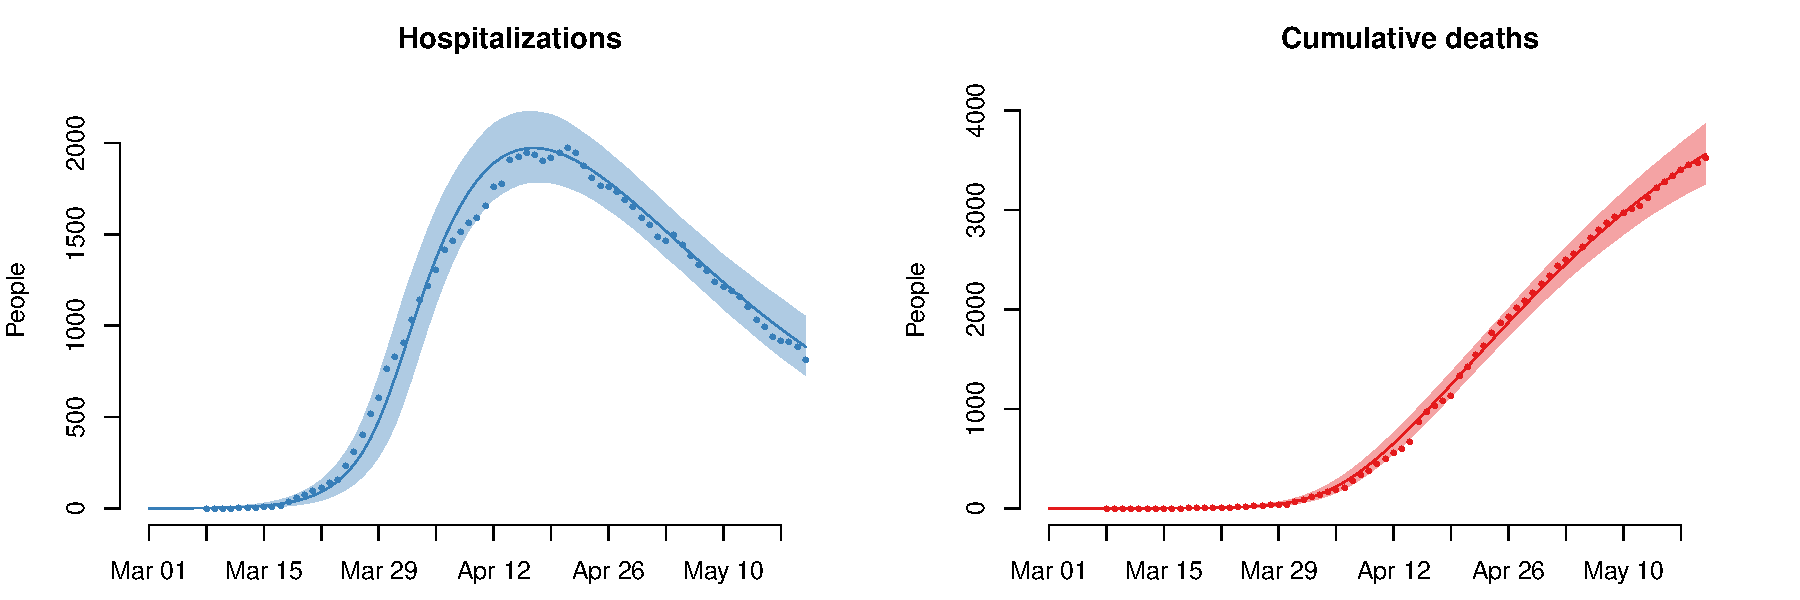
\includegraphics[width=\textwidth]{figures/calibration.pdf}
\caption{Model projections of current hospitalizations and cumulative deaths, with observed data, from March 1 to May 20, 2020. Solid lines show average model projections and the intervals show 90\% uncertainty regions.  Observed data are overlaid as solid dots.} 
\label{fig:calibration}
\end{figure}


\subsection*{Projections under slow reopening} 

Figure \ref{fig:slow} shows projections of daily incidence, cumulative incidence, hospitalizations, and deaths under a ``slow'' reopening scenario. At one-month intervals, 10\% of the suppressed contact (relative to March 1 baseline) is released. In these projections, \comment{incidence...} Hospital census continues its gradual decline through June, flattening in July, and rising again in August. Deaths rise slowly, with the greatest increases occurring in August. 


\begin{figure}
\centering
\comment{slow reopen placeholder}
%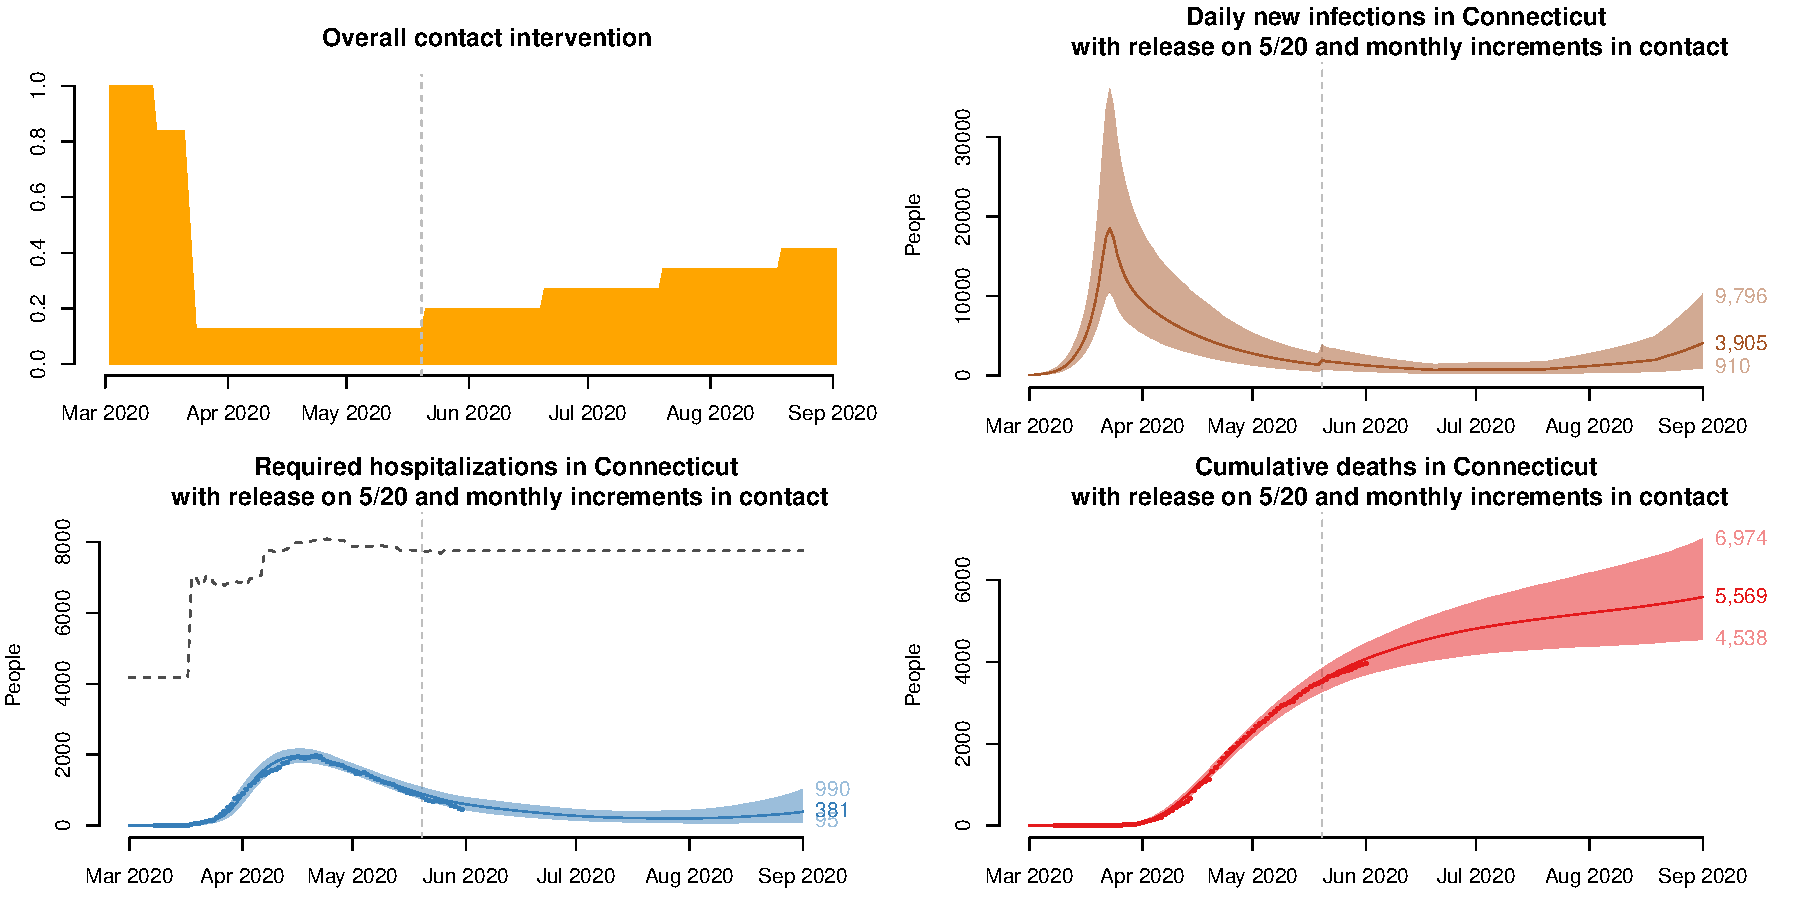
\includegraphics[width=\textwidth]{figures/slow.pdf}
\caption{Projections under a ``slow'' reopening scenario. }
\label{fig:slow}
\end{figure}



\subsection*{Projections under fast reopening} 

Figure \ref{fig:fast} shows projections of daily incidence, cumulative incidence, hospitalizations, and deaths under a ``fast'' reopening scenario. At one-week intervals, 10\% of the suppressed contact is released.   

\begin{figure}
\centering
\comment{fast reopen placeholder}
%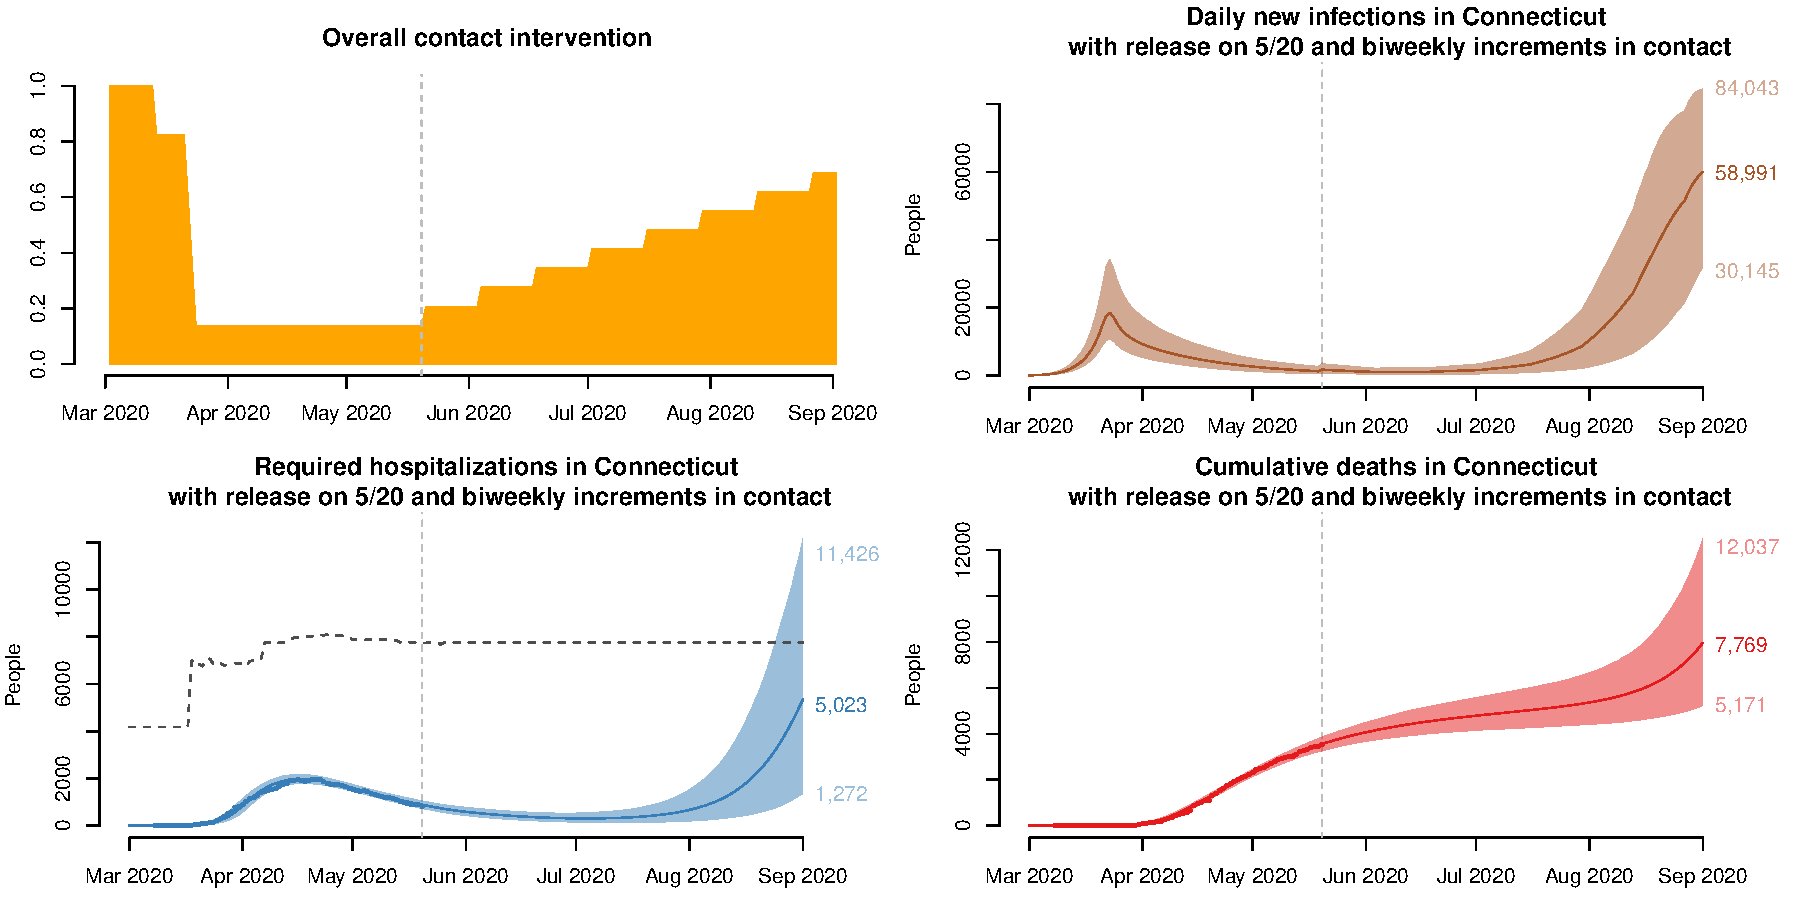
\includegraphics[width=\textwidth]{figures/fast.pdf}
\caption{Projections under a ``fast'' reopening scenario. }
\label{fig:fast}
\end{figure}




%%%%%%%%%%%%%%%%%%%%%%%%%%%%%%%%%%%%


\section*{Implications}

The COVID-19 outbreak in Connecticut is currently declining, with hospitalization census and the number of deaths per day decreasing since mid April.  However, as the state reopens, there is a risk that increased contact will result in a second wave of COVID-19 transmission, leading to an increase in hospitalizations and deaths.  If contact remains low throughout the summer, with only minimal increases due to reopening, a possible second wave will be blunted and pushed into the future.  On the other hand, if contact returns quickly to a level seen in early March, then a resurgence in hospitalizations and deaths is likely to occur in August.  Importantly, Connecticut decision-makers may not know which of these scenarios is occurring until sometime in July.  


\subsection*{Risk of resurgence following reopening} 

Projections under high asymptomatic fraction or fast reopening suggest that increased transmission following the May 20 reopening may result in a rapid rise new infections in June and July, followed by an increase in hospitalizations during August, and a subsequent increase in deaths following soon after.  It is important to note that if transmission increases immediately following reopening, the first indications of this increase would not be apparent until mid to late July, as the first post-reopen infections become hospitalizations.  Therefore it is important that public health authorities closely monitor new hospitalizations as well as hospital census for signs of increased numbers COVID-19 cases requiring healthcare.   


\subsection*{Importance of testing to detect changes in incidence}

Enhanced viral testing, especially of asymptomatic individuals, may help provide an early warning of increased transmission following reopening.  Because there is a roughly 3-week lag between a new infection and possible hospitalization of the infected individual, widespread and frequent testing could detect increased incidence before the first new symptomatic cases present to the hospital.  

Daily new infections are not observable, but can be estimated...

Figure \ref{fig:dailyincidence} shows daily incidence 




\begin{figure}
\centering
% \includegraphics...
\caption{\comment{show daily incidence}}
\label{fig:dailyncidence}
\end{figure}




\subsection*{Model projections to inform seroprevalence studies}

Expanded antibody testing in Connecticut could dramatically improve knowledge about seroprevalence -- the proportion of people in Connecticut who have evidence of prior COVID-19 infection. If this proportion were more precisely known, the fraction of infected individuals who are asymptomatic could be estimated with greater certainty,   This knowledge would reduce uncertainty in future projections.  In order to design a valid seroprevalence study, researchers need to calculate the minimum sample size required to obtain an estimate that is sufficiently precise, requiring an estimate of the proportion of individuals who would test positive for antibodies. 


Model projections offer the opportunity to evaluate this quantity on future dates during which a proposed seroprevalence study might be conducted.  Figure \ref{fig:cumincidence} shows projections of cumulative incidence among alive non-hospitalized individuals who might be sampled and tested in a seroprevalence taking place on future dates.  

\comment{Olya, can you write a few sentences about how knowing cumulative incidence would help us learn the infection fatality ratio, asymptomatic fraction, etc? }


\begin{figure}
\centering
% \includegraphics...
\caption{\comment{show cumulative alive incidence and current prevalence }}
\label{fig:cumincidence}
\end{figure}





\subsection*{Uncertainty about transmissibility in children}

Children are unlikely to experience severe symptoms when infected with COVID-19. For this reason, epidemiologists do not yet know how transmissible school-age children may be when they are infected, and epidemiological studies have provided conflicting evidence regarding viral shedding and transmissibility in children. Because Connecticut closed K-12 schools approximately only one week before the stay-at-home order took effect, we do not have specific information about the isolated effect of closing schools on the subsequent reduction in transmission.  If child care and summer camps reopen as planned at the end of June [ref], we may be able to gain information about transmissibility in children from any subsequent increase in cases observed among people who are more likely to be symptomatic.  This information will be useful in projecting COVID-19 dynamics in the Fall if K-12 education will take place in person. 


\comment{Olya, can you write a few sentences and give references for what we know and don't know about transmission in children?}



%%%%%%%%%%%%%%%%%%%%%%%%%%%

\textbf{About this report}: The most recent version of this report is available from [Project web page] with source at \url{https://github.com/fcrawford/covid19_ct_report1}. Release versions are hosted at \url{https://github.com/fcrawford/covid19_ct_report1/releases}. 


%%%%%%%%%%%%%%%%%%%%%%%%5

\textbf{Disclosures}: FWC is a member of the Reopen Connecticut Steering Committee.  The authors report no conflicts of interest. 

%%%%%%%%%%%%%%%%%%%%%%%%5


\textbf{Acknowledgements}: We are grateful to
Matthew Cartter,
Joshua Geballe,
Gregg S. Gonsalves,
Alexander Karnal,
Harlan Krumholz,
Albert Ko, 
and
Daniel Weinberger
for helpful comments and feedback. 


%%%%%%%%%%%%%%%%%%%%%%%%%%%%%

\bibliographystyle{unsrtnat}
\bibliography{covid19}


\end{document}

